\subsection{Use Case - Edinburgh Cancer Gateway}

\noindent
In the use case that we consider, we developed a dashboard to help the oncologist observe, monitor, and analyse the patients' condition as well as the chemotherapy treatments which might improve the well-being and survival rate of the patients. Our ultimate aim is to build a \emph{toxicity predictors model} to predict toxicity of the treatment based on treatment history and feedback from patients. 
\begin{figure}[t!]
    \centering
    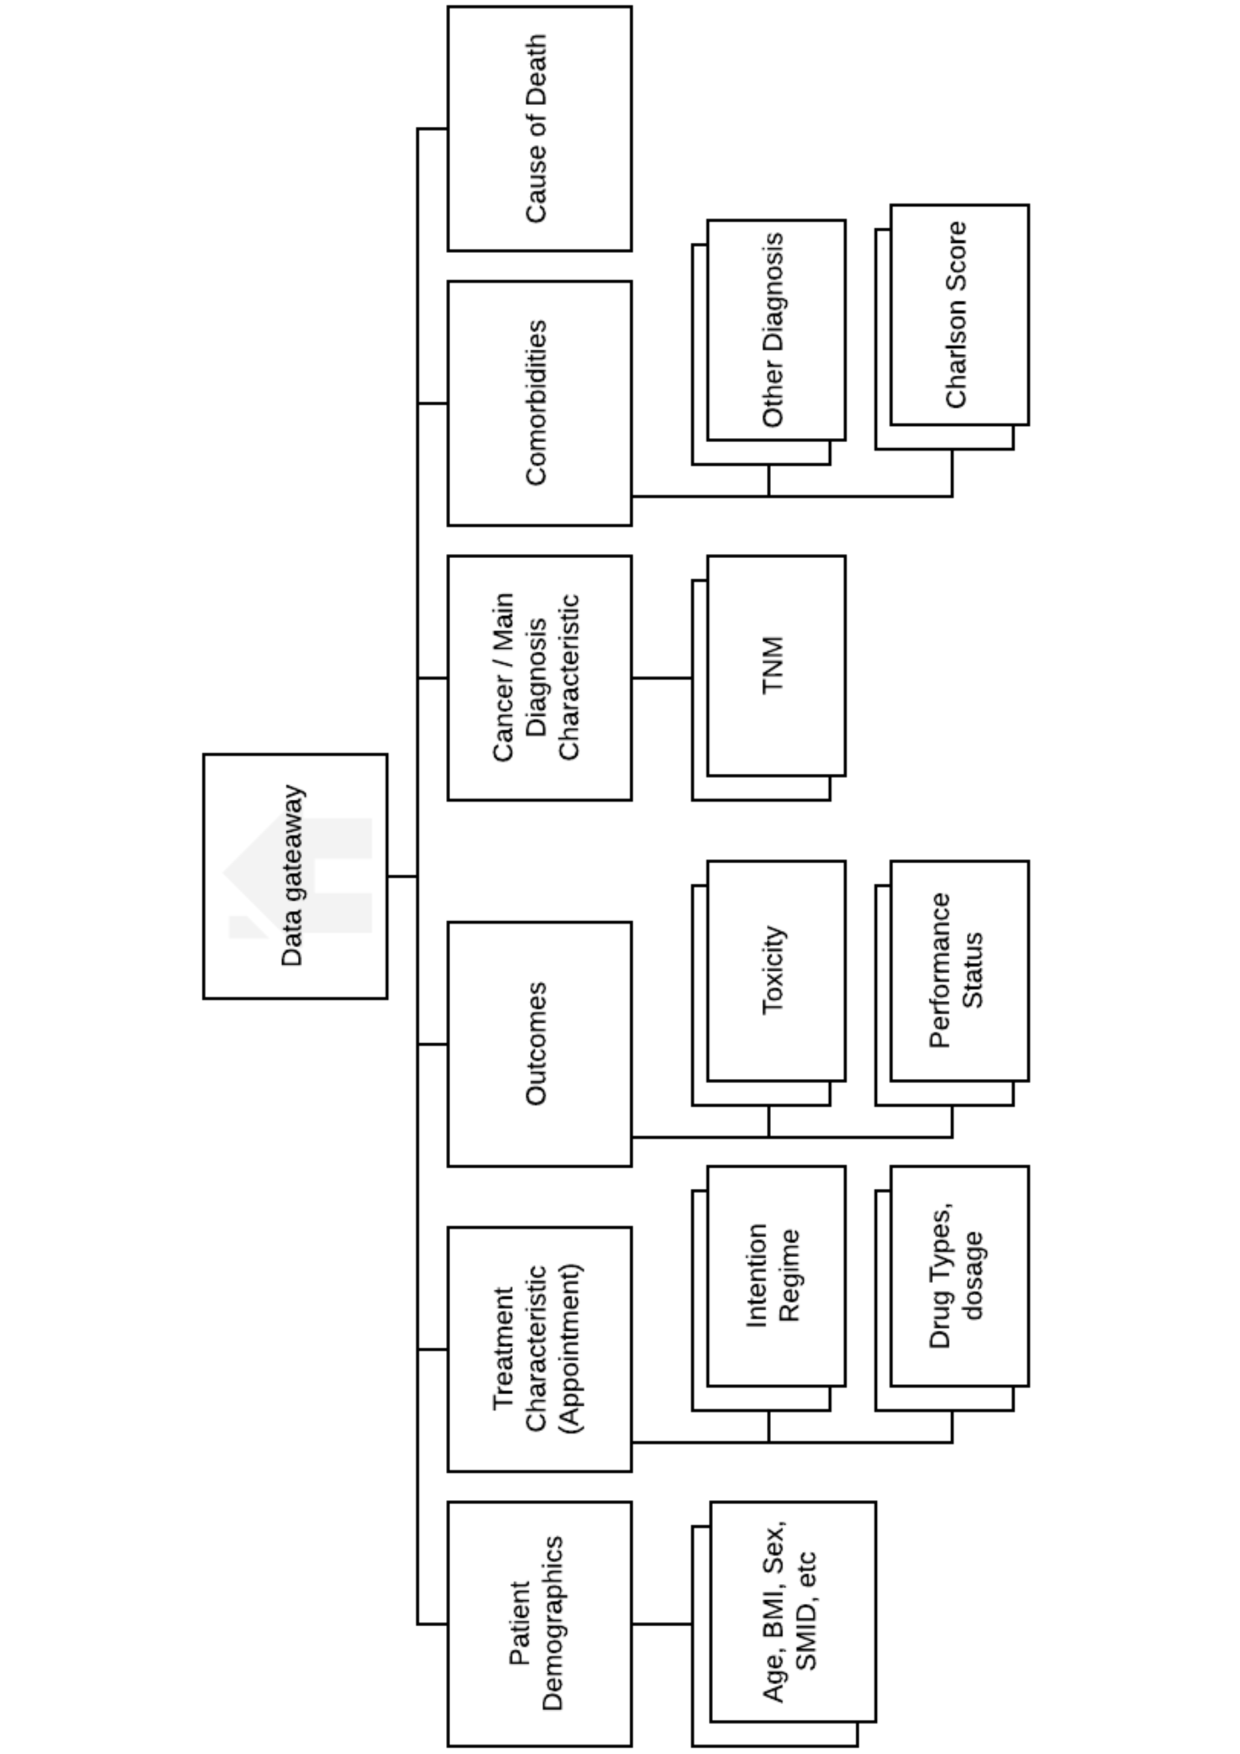
\includegraphics[angle=-90,width=0.45\textwidth]{images/ECG.pdf}
    \caption{Database Structure for Training the Toxicity Predictor Model}
    \label{fig:ECG}
\end{figure}
Figure~\ref{fig:ECG} shows the data structure we use for training the toxicity predictors model. We extracted the data during the initial step for training the machine learning models from three main databases (i.e., Chemocare, Trak, and Oncology DB) in the Edinburgh Cancer Centre (ECC). The data contains the information on treatment cycles, recorded side effects (here, toxicity level), comorbidities, and various observations concerning breast cancer patients for three years (from 2014 to 2016). The extraction has data for 51661 treatments, of which 13030 are of breast cancer treatments. There are 933 unique patients, and some patients may have two or three different treatments/regimes. Each regime has several cycles ranging from one to more than 50 cycles (e.g., 85) [cite: On Predicting the Outcomes of Chemotherapy Treatments in Breast Cancer].

\subsection{Evaluation Framework}

\subsection{Smart Patient Records}

\subsection{Data Fabrication}

\subsection{Blockchain}

\subsection{Authentication}

\subsection{Data Analytics}

%Need 2-3 pages on use case.